\chapter{Introducción}

\section{Introduccón}
Este documento es el reporte técnico final del trabajo terminal titulado “Sistema de realidad virtual del cuerpo humano para el estudio del sistema digestivo” con número de registro TT: 2019-A104.

En el presente capítulo se habla del problema identificado, por qué se considera como tal y cómo es que se ayudó a resolver el problema planteado mediante la ingeniería en sistemas computacionales. También se menciona que se obtiene al concluir con este trabajo terminal, tales como el prototipo del sistema.

En el capítulo \textbf{II Análisis} se mostrarán todos los diagramas y documentos generados al analizar y generar un diseño del sistema que se estará desarrollando. Aquí se encuentra la arquitectura general del sistema, y los modelos gráficos de apoyo presentados en el Análisis Estructurado Moderno.

En el capítulo \textbf{III Diseño} se describe el trabajo generado en el desarrollo del documento hasta el mes de mayo de 2020 para TT2.

En el capítulo \textbf{IV Verificación y Pruebas} se muestran pruebas hechas sobre las implementaciones del sistema siguiendo un guión para la prueba.

En el capítulo \textbf{V Conclusión} se muestran los resultados obtenidos y experiencias para mejorar el proceso, así como la vertiente para continuar con el trabajo y las conclusiones del integrante.

Finalmente, se encuentran las referencias de todos los recursos empleados para dar soporte y estructura a este Trabajo Terminal, y en los apéndices se anexan elementos extra que dan información más detallada sobre lo que aquí fue realizado.

\section{Detección del problema} 

Durante 2019 se entrevistó al Dr. Rios Macias jefe del área de morfología de la Escuela Superior de Medicina del Instituto Politécnico Nacional y comentó que “los medios que se utilizan para el estudio del cuerpo humano principalmente son medios impresos tradicionales, así como el uso de cuerpos para su disección y análisis posterior”. El uso de cuerpos para su disección tiene un alto costo que incluye el mantenimiento del cuerpo en las instalaciones, el mantenimiento de las instalaciones, y la inhumación de los cuerpos.
\\
\newline
\section{Propuesta de Solución}

Se elaboró un sistema de realidad virtual del sistema digestivo del cuerpo humano que permite interactuar con modelos tridimensionales. La intención es sentar las bases para un sistema de apoyo al aprendizaje que sea más práctico \cite{moore1995learning}, sin sustituir a ningún método de estudio tradicional.
\\
\newline
\section{Justificación}
\label{just}

El sistema tiene los siguientes beneficios para docentes y alumnos: 
\begin{itemize}
\item Fuentes confiables. Se usaron textos médicos y sitios web especializados
\item Uso de realidad virtual\cite{norton1994integrating}.
\end{itemize}

El sistema es un ejemplo de cómo se pueden actualizar las herramientas educativas, como las que se pueden encontrar en Statista \cite{web1}, y que representan un mercado de aproximadamente 18.8 mil millones de dólares para el año 2020. Además, Nielsen\cite{web2} muestra los datos sobre la expectativa de adopción de la realidad virtual y aumentada en diferentes continentes, como se muestra el Figura 1 y 2.

\begin{figure}[H]
	\begin{center}
 		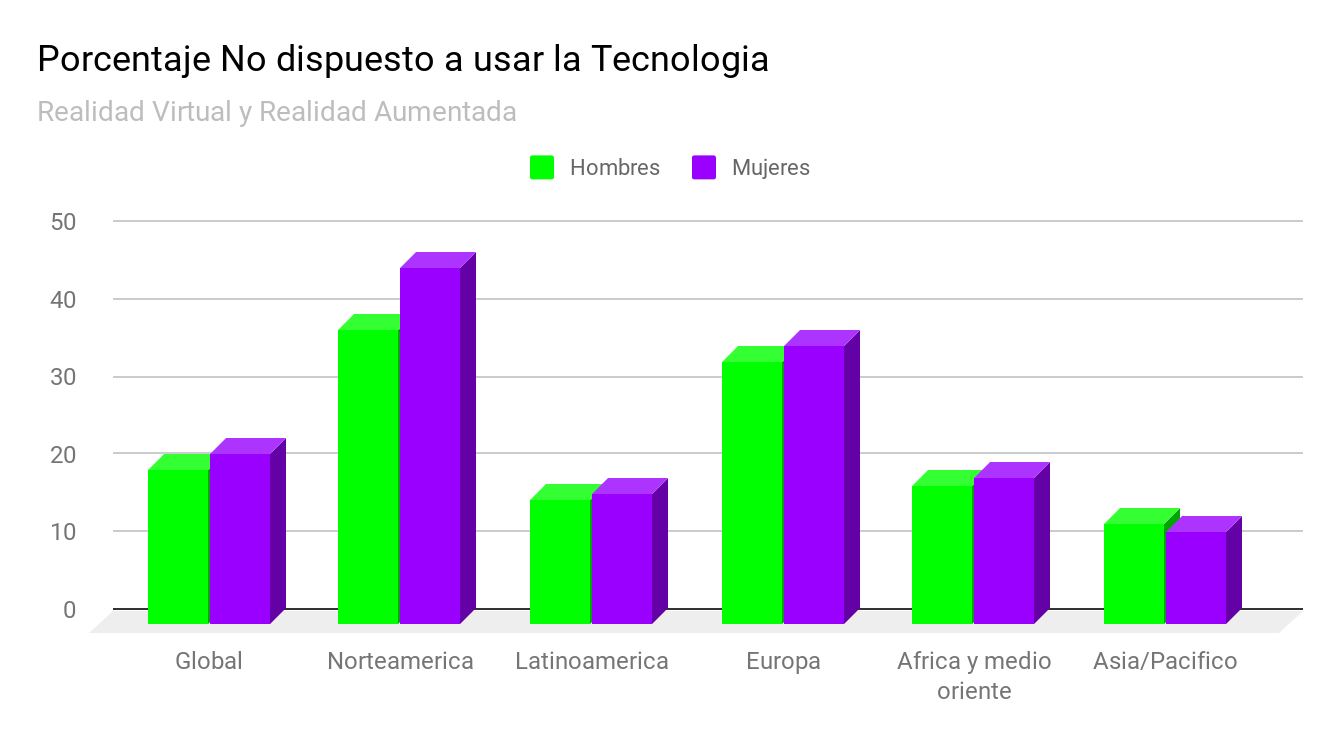
\includegraphics[width = 0.7\textwidth]{source/images/image2.png}
 		\captionof{figure}{\label{fig:graph1}Disposición de los consumidores a nivel mundial para usar la realidad virtual y aumentada si esta se encuentra disponible en los próximos 2 años (2020 -2021)}
	\end{center} 
\end{figure}

\begin{figure}[H]
	\begin{center}
 		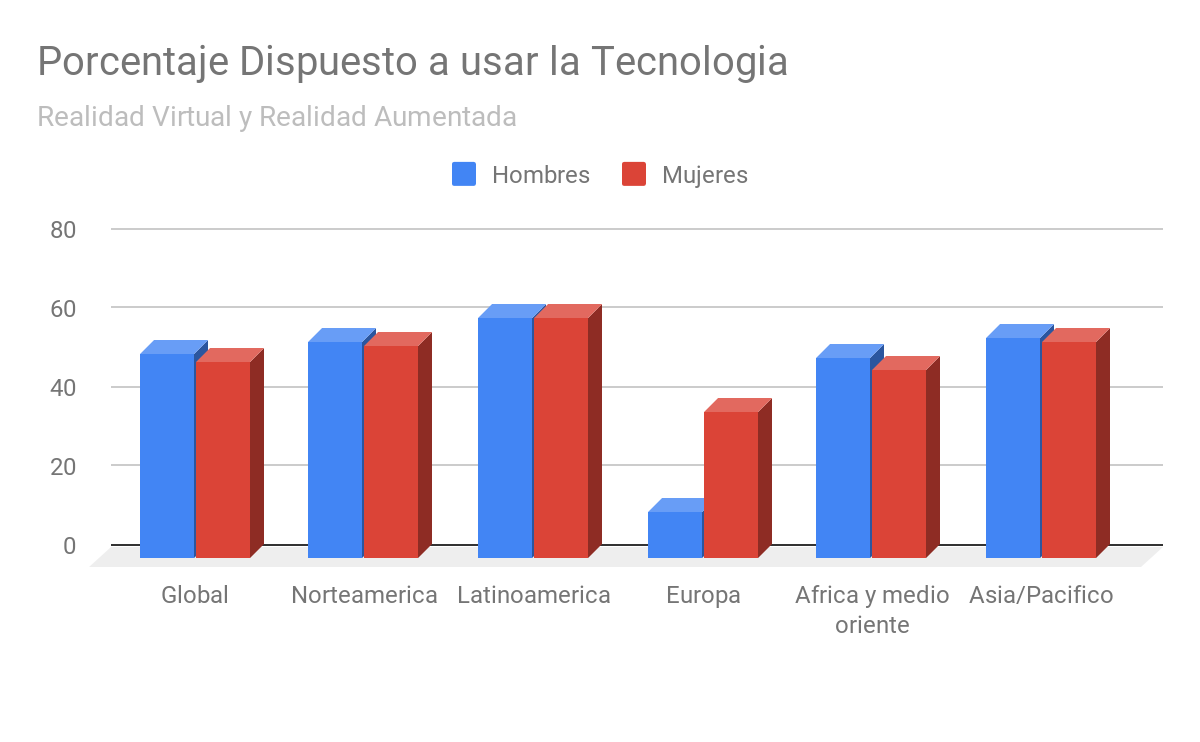
\includegraphics[width = 0.7\textwidth]{source/images/image10.png}
 		\captionof{figure}{\label{fig:graph2}Disposición de los consumidores a nivel mundial para no  usar la realidad virtual y aumentada si esta se encuentra disponible en los próximos 2 años(2020 -2021)}
	\end{center} 
\end{figure}

A medida que crece el consumo de software, multimedia y videojuegos se aumentará la disponibilidad de sistemas como el que se propone en este trabajo terminal.
\\

\section{Objetivos del Trabajo}
Objetivo es analizar, diseñar, desarrollar y probar un sistema de demostración que utiliza la tecnología de Realidad Virtual, para ofrecer una experiencia orientada al estudio de la anatomía y morfología del cuerpo humano, específicamente del sistema digestivo.
\newline

\subsection{Objetivos Específicos}
Para lograr el objetivo se identificaron los siguientes objetivos específicos:
\newline
\begin{itemize}
\item Investigar en fuentes confiables sobre el sistema digestivo.
\item Analizar, diseñar, desarrollar y probar un entorno de Realidad Virtual para la interacción.
\end{itemize}

\section{Población Objetivo}
De acuerdo a un estudio de Ericsson ConsumerLabe\cite{web3}, en el año 2020 un tercio de los consumidores serán usuarios de Realidad Virtual. Ya desde 2017 se había explorado el nivel de interés de los consumidores en Realidad Virtual\cite{web4} con su potencial de reunir gente de todo el mundo y crear un experiencia más profunda, personalizada y enriquecida.\\
\newline
De todos los interesados en la Realidad Virtual se toma a los estudiantes de educación superior del área de medicina, particularmente a 180\cite{ofi1}  estudiantes de la Escuela Superior de Medicina del Instituto Politécnico Nacional de entre 18 y 24 años de edad. Además se espera que los usuarios objetivo tengan las siguientes características\cite{web5} específicamente:\\
\newline
\begin{itemize}
\item Disposición para el aprendizaje con nuevas tecnologías de la información.
\item Conocimientos sólidos en las áreas de biología, física, química; y en forma idónea conocimientos básicos de las etimologías grecolatinas e idioma inglés, que le facilitarán la comprensión y dominio de los conceptos utilizados en las asignaturas básicas y clínicas.
\item No ser propenso a sufrir cinetosis.
\end{itemize}

\section{Productos logrados}
Se logró crear un software (demostración), de una experiencia demostrativa en realidad virtual. El sistema muestra características y elementos del sistema digestivo y permite la participación de un usuario utilizando una misma computadora de forma local. Se usan los controles Oculus Touch ® así como el visor de Realidad Virtual Oculus Rift ®. También se redactó el presente reporte técnico.

\section{Definiciones}
Estas son las definiciones más importantes para el presente trabajo terminal

\subsection{Realidad Virtual}
Algunos autores definen así la Realidad Virtual.\\
\newline
\textit{“La realidad virtual (RV) es una simulación tridimensional generada o asistida comúnmente por computadora de algún aspecto del mundo real o ficticio, en el cual el usuario tiene la sensación de pertenecer a ese ambiente sintético o interactuar con él”}\cite{web6}\\ 
\textbf{Corrado Padila Érica}\\
\newline
“Realidad Virtual: gráficos 3D en entornos inmersivos que usan I/O
artefactos como guantes, cascos, etc. en busca de mayores grados de iteración
con el ambiente virtual”\cite{web7}\\ 
Lozano Miguel, Calderón\\
\newline
"Realidad Virtual es una forma en que los seres humanos puedan
visualizar, manipular e interactuar con las computadoras y datos extremadamente
complejos".\cite{web8}\\
Isdale, Jerry\\
\newline
“Un sistema interactivo capaz de crear una simulación que implique a varios de los sentidos del ser humano, generados por una computadora, explorable, visualizable y manipulable en tiempo real; este bajo la forma de imágenes y sonidos, estos, dando la sensación de presencia en el entorno generado”\cite{web9}\\
Levis, Diego\\
\newline
Esta última ha sido la definición que se ha tomado para el desarrollo del proyecto del trabajo terminal, asimismo se puede concluir que todos los autores coinciden en que la realidad virtual es un mundo simulado en el que el usuario puede interactuar en tiempo real por medio
de dispositivos o computadoras que logran un efecto artificial e inmersivo en el que se pueden manipular objetos.

\subsection{Producto Multimedia}
Los productos multimedia se pueden clasificar en dos categorías: productos interactivos y no interactivos. Los productos no interactivos también se pueden clasificar en productos estáticos como carteles, logotipos, folletos, modelos estáticos 3D, etc., y productos basados en el tiempo. \cite{engels2002object,sauer2001uml}.\\ 
\newline
Los productos multimedia interactivos son aplicaciones de software que contienen productos multimedia\cite{miranda2017diseno} (es decir, aplicaciones basadas en eventos como juegos, aplicaciones web basadas en multimedia y materiales de aprendizaje multimedia basados en interactividad).  La figura \ref{fig:diag1} a continuación ilustra los tipos de productos multimedia.\\
\begin{figure}[H]
	\begin{center}
 		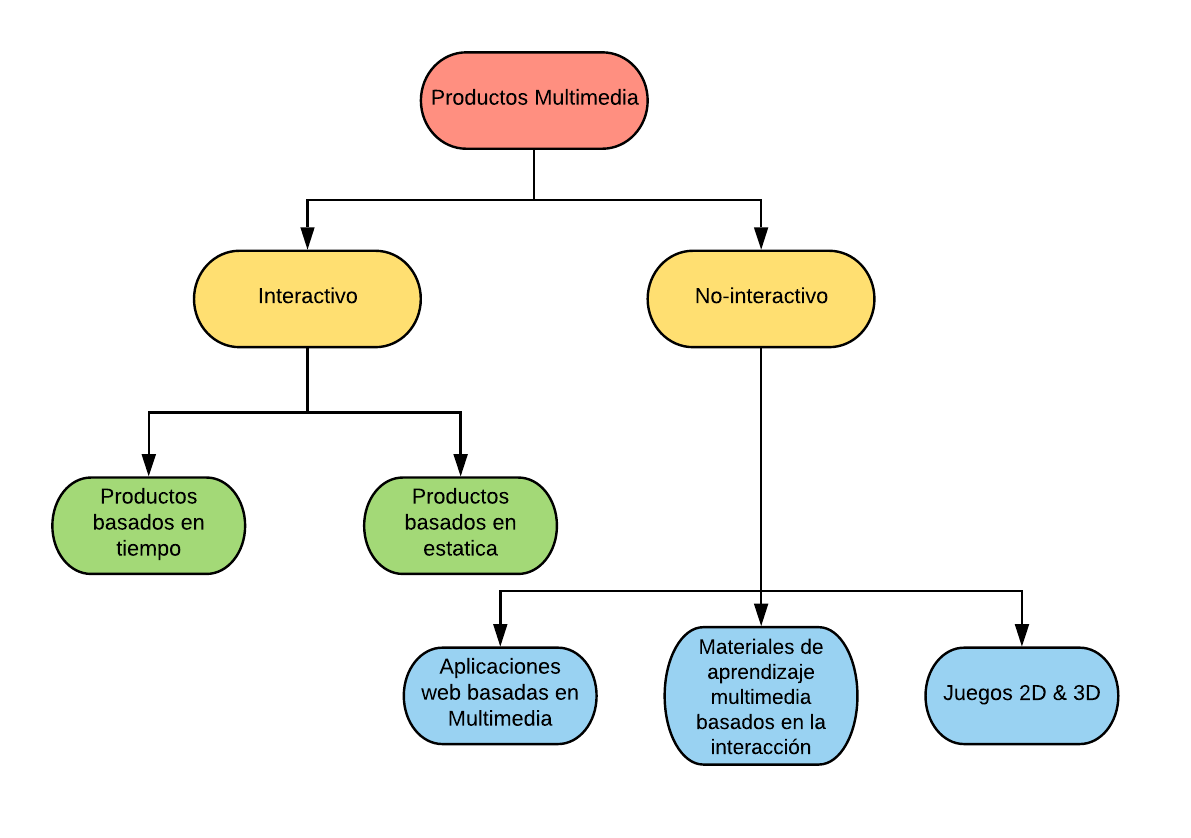
\includegraphics[width = 1\textwidth]{source/images/image52.png}
 		\captionof{figure}{\label{fig:diag1}Tipos de productos multimedia} 
	\end{center} 
\end{figure}

Un sistema multimedia se puede analizar desde tres puntos:
\begin{itemize}
\item La vista externa. La forma en que el usuario interactúa con el producto.
\item Flujo de acciones. El orden en que se muestran los marcos de los modelos a los usuarios. \cite{aleem2016game,cartwright1996pre}.
\item  Los roles de los usuarios. La interacción con productos multimedia.
\end{itemize} 
El cuadro \ref{tab:tab1} resume los tipos de productos multimedia y sus características.

\begin{longtable}[c]{
>{\columncolor[HTML]{EFEFEF}}c ccc}
\cellcolor[HTML]{C0C0C0} &
  \multicolumn{3}{c}{\cellcolor[HTML]{C0C0C0}\textbf{Características Multimedia}} \\
\multirow{-2}{*}{\cellcolor[HTML]{C0C0C0}\textbf{\begin{tabular}[c]{@{}c@{}}Tipos de productos\\  multimedia\end{tabular}}} &
  \cellcolor[HTML]{C0C0C0}\textbf{\begin{tabular}[c]{@{}c@{}}Vista \\ \\ Externa\end{tabular}} &
  \cellcolor[HTML]{C0C0C0}\textbf{\begin{tabular}[c]{@{}c@{}}Flujo \\ \\ de acciones\end{tabular}} &
  \cellcolor[HTML]{C0C0C0}\textbf{\begin{tabular}[c]{@{}c@{}}Roles de \\ \\ los Usuarios\end{tabular}} \\
\endfirsthead
%
\endhead
%
\hline
\endfoot
%
\endlastfoot
%
\textit{Productos estáticos} &
  Un cuadro &
  Sin acciones &
  Pasivo (ver/leer) \\
\textit{\begin{tabular}[c]{@{}c@{}}Productos basados\\  en tiempo\end{tabular}} &
  Múltiples cuadros &
  Secuencia &
  Pasivo(mirar) \\
\textit{Productos interactivos} &
  Impulsado por eventos &
  \begin{tabular}[c]{@{}c@{}}Secuencia, Selectiva,\\  Interactiva e\\  Impulsada por eventos\end{tabular} &
  Activo(Realiza eventos) \\ \hline
\caption{Características de los productos multimedia.}
\label{tab:tab1}\\
\end{longtable}
Para este trabajo, el sistema que se propone es una producto interactivo.

\section{Estado del Arte}
A continuación se muestran algunos de trabajos académicos desarrollados en México y fueron comparados con el trabajo planeado. Como comparativa y de forma ilustrativa del sector académico.\\
\newline
\begin{enumerate}
\item TT No. 2014-A058 “Sistema para la orientación de los efectos sobre la espalda humana en pacientes con sobrepeso”\cite{tt1}
\item TT No. 2012-B055 “Laboratorio Virtual del cuerpo humano 3D con asistente de ayuda en línea para el nivel superior bajo el paradigma de Educación Basada en Web con tecnologías de Web Semántica”\cite{tt2}
\item TT No. 2014-B035 “Simulación en Tercera Dimensión del Sistema Circulatorio de los Cánidos para el uso Educativo”\cite{tt3}
\item TT No. 2014-B039 “Simulación de una Línea del Metro con Realidad Virtual”\cite{tt4}
\item Tesis que para optar por el grado de Maestro en Ciencia e Ingeniería de la Computación, Sistema de seguimiento de movimiento de las extremidades superiores basado en sensores inerciales para rehabilitación en realidad virtual.\cite{mastersthesis1}
\item Adecuación educativa de la realidad virtual como herramienta didáctica para el proceso enseñanza-aprendizaje / tesis que para obtener el título de Licenciado en Pedagogía, presenta Maria de la O García Noriega; asesor Lucina Moreno Valle Suárez.\cite{te1}
\end{enumerate}
Así mismo se ha encontrado software propietario desarrollado por empresas privadas los cuales son los siguientes.\\
\begin{itemize}
\item The Body VR: Anatomy Viewer es la única herramienta de visualización de Realidad Virtual disponible en el mercado que se basa en datos médicos específicos del paciente (por ejemplo, MRI, CT, PET) y cumple con los estándares DICOM. Proporciona simulaciones de R.V. anatómicas en tiempo real para visualizar diagnósticos médicos, ilustrar el impacto de los procedimientos y tratamientos, y crear una toma de decisiones más educada.\
\begin{figure}[H]
	\begin{center}
 		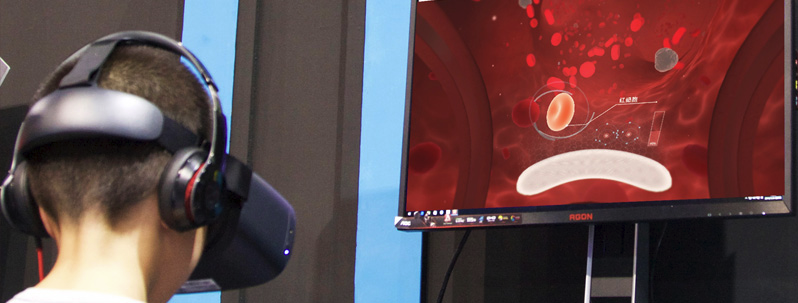
\includegraphics[width = 0.5\textwidth]{source/images/image9.png}
 		\captionof{figure}{\label{fig:ea1}Software “The Body VR” en uso.}
	\end{center} 
\end{figure}
\item Anatomyou VR: Estructuras anatómicas fotorrealistas, modeladas en colaboración con RenderArea, validadas por expertos clínicos y certificadas por personal capacitado en  Tecnologías Médicas de la Universidad de Las Palmas de Gran Canaria.
\begin{figure}[H]
	\begin{center}
 		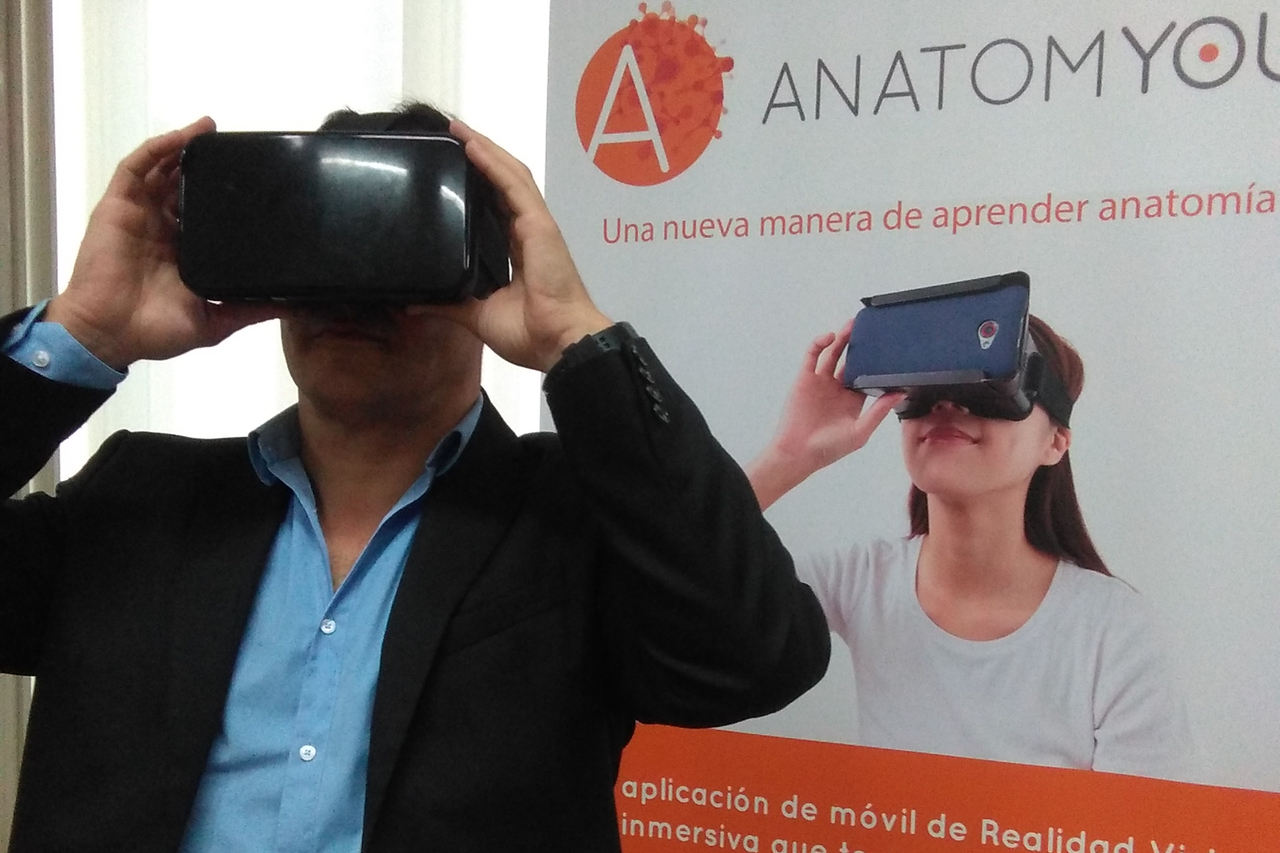
\includegraphics[width = 0.5\textwidth]{source/images/image59.png}
 		\captionof{figure}{\label{fig:ea2}Pancarta promocional de “Anatomyou VR}
	\end{center} 
\end{figure}
\item Biodigital Anatomy: El cuerpo tridimensional más completo, científicamente preciso e interactivo jamás ensamblado. Anatomía masculina y femenina, en los detalles básicos (gratuitos) y profesionales. Cada sistema está completamente segmentado, etiquetado y direccionable para una fácil configuración que satisfaga cualquier necesidad educativa.
\begin{figure}[H]
	\begin{center}
 		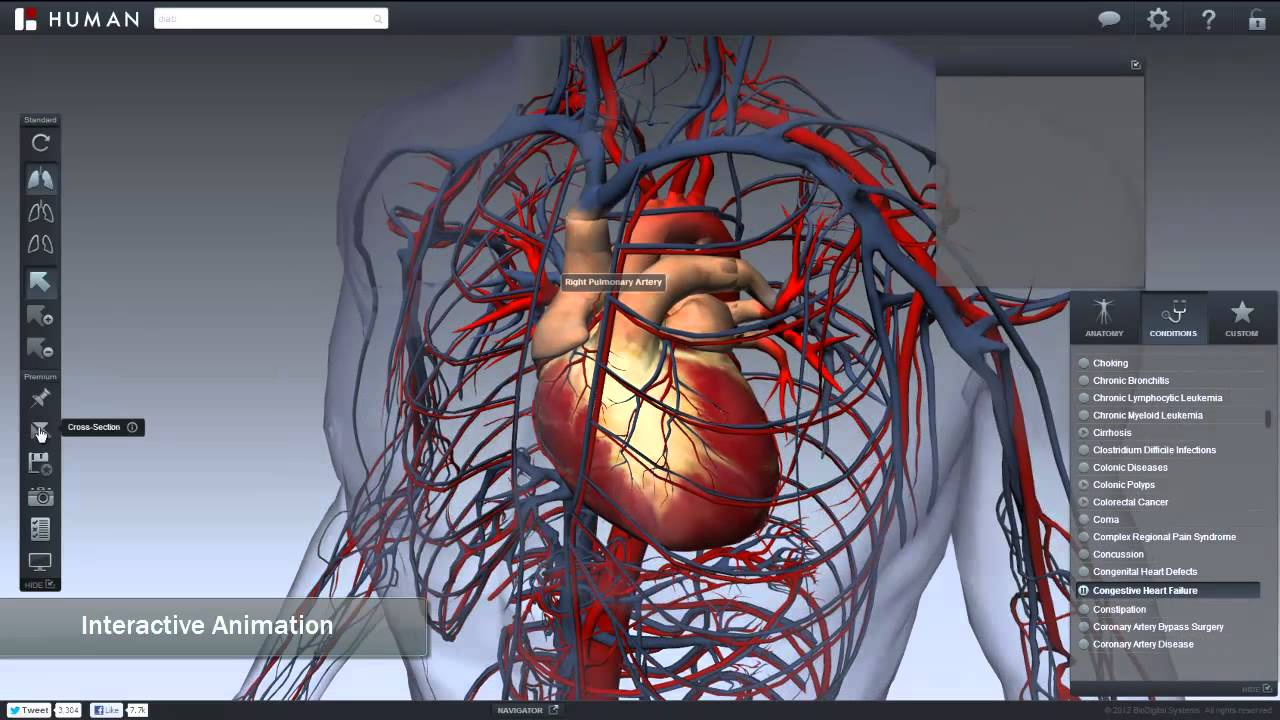
\includegraphics[width = 0.5\textwidth]{source/images/image18.png}
 		\captionof{figure}{\label{fig:ea3}Interfaz del software de Biodigital Anatomy}
	\end{center} 
\end{figure}
\item 3D Organon VR Anatom: 3D Organon es un completo atlas anatómico que presenta los 15 sistemas del cuerpo humano. Incluye más de 4,000 estructuras y órganos anatómicos realistas y más de 160 correlaciones clínicas encontradas por sistema del cuerpo.
\begin{figure}[H]
	\begin{center}
 		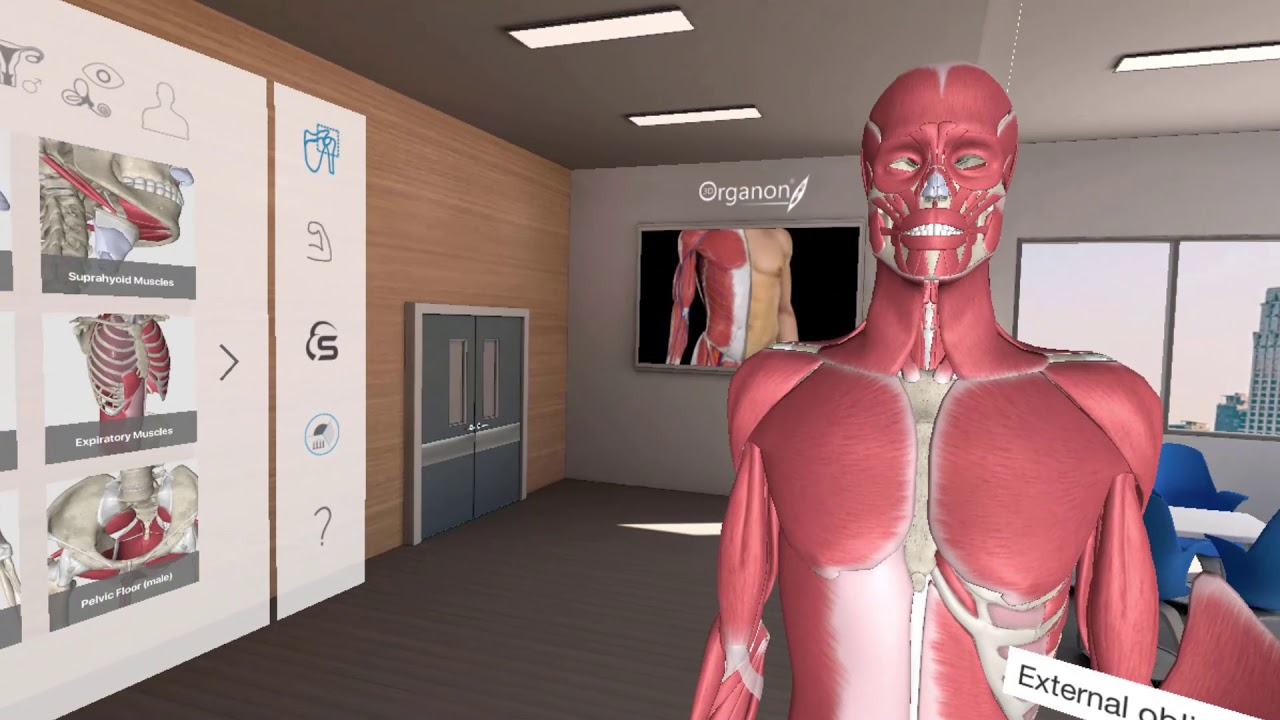
\includegraphics[width = 0.5\textwidth]{source/images/image5.png}
 		\captionof{figure}{\label{fig:ea4}Interfaz del software de 3D organon VR Anatom}
	\end{center} 
\end{figure}
\end{itemize}

%%
%% Este es uno de los puntos más críticados del trabajo,
%% la falta de metodología, así que es donde hay que revisar más.
%% Falta:
%%    - Colocar las referencias a OpenUp y RUP.
%%    - Escribir el acrónimo de RUP.
%%    - Explicar como se adaptó OpenUP
%%    - Mostrar la comparativa de OpenUP vs OpenUP adaptado a este TT.
%%
\section{Metodologías}
Se siguió como modelo de desarrollo a la metodología OpenUp [ 24 ], 
que está basada en RUP. 
OpenUP es extensible y se usó como base, ya que se adaptó al desarrollo de este proyecto.
La figura \ref{fig:me1} muestra el ciclo de vida iterativo de OpenUP.
\begin{figure}[H]
	\begin{center}
 		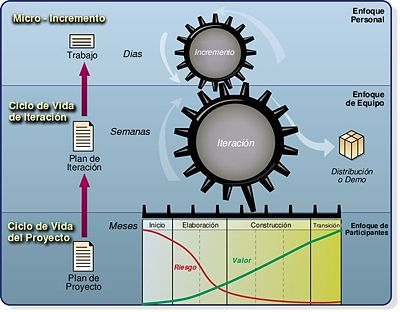
\includegraphics[width = 0.5\textwidth]{source/images/image70.png}
 		\captionof{figure}{\label{fig:me1}Ciclo de Vida Iterativo de OpenUP}
	\end{center} 
\end{figure}

OpenUP está organizado en contenido y proceso, con cuatro fases concepción o creación del proyecto, preparación o elaboración detallada del proyecto, construcción y transición.\\

Además también se consideró la Metodología de ingeniería de software multimedia que tiene como fases, requisitos y preproducción, diseño y producción, validación y Postproducción y evolución, como se puede ver en la figura \ref{fig:me2}

\begin{figure}[H]
	\begin{center}
 		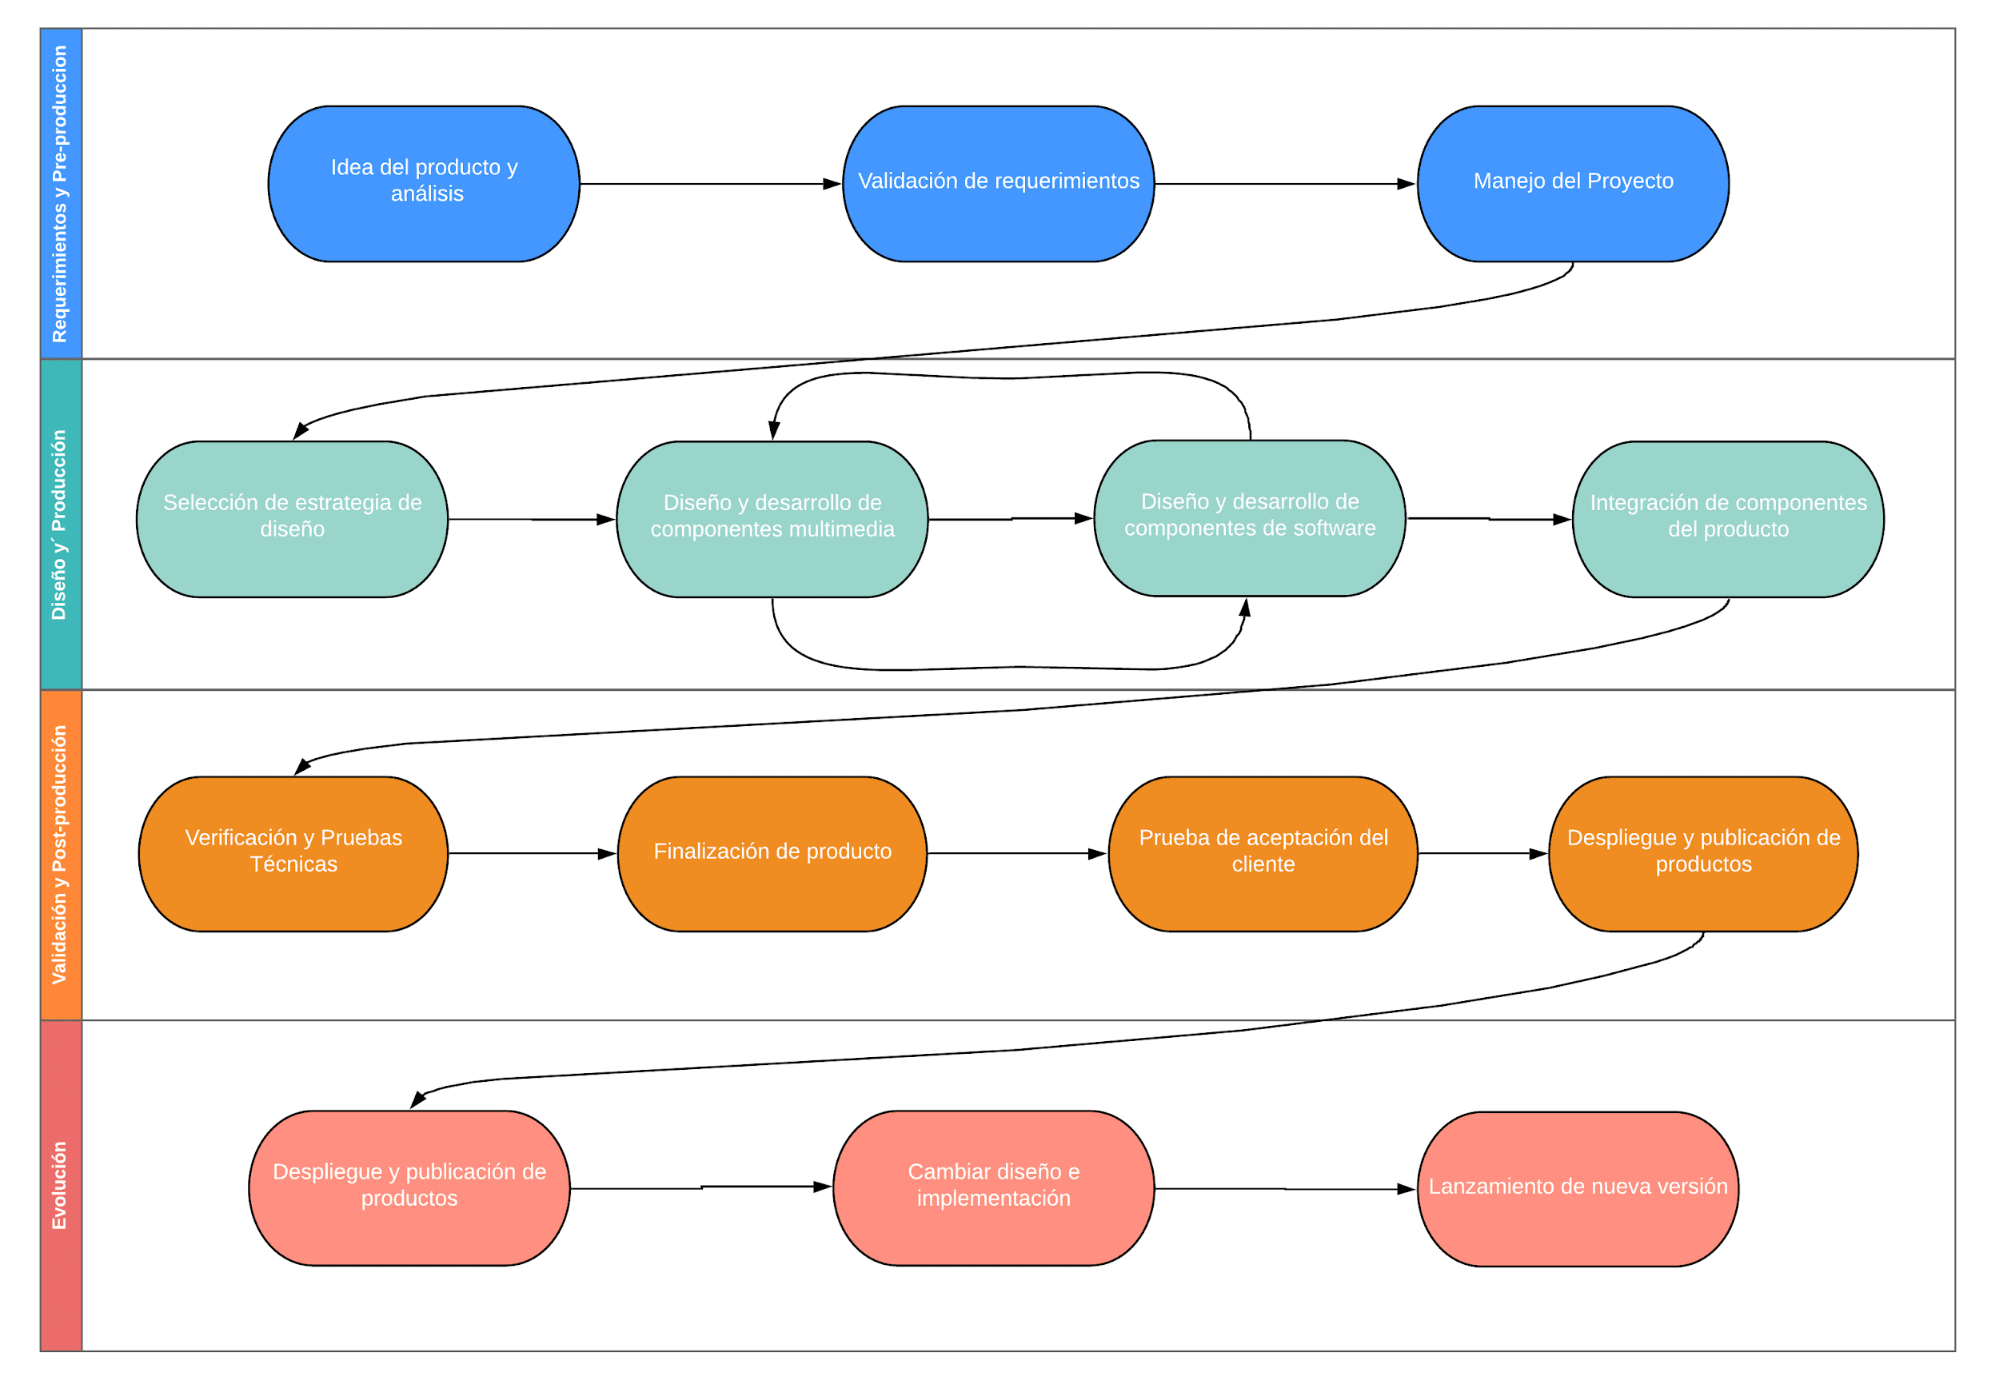
\includegraphics[width = 1\textwidth]{source/images/image50.png}
 		\captionof{figure}{\label{fig:me2}Fases de la Metodología de ingeniería de software multimedia}
	\end{center} 
\end{figure}

También se tomó como referencia a Git-flow\cite{driessen2010successful} que es un modelo de ramificación que consiste en separar cada característica en su propia rama de desarrollo. Se utiliza una versión simplificada del modelo\cite{krusche2014introduction} compuesta por tres tipos principales de ramas.\\
\begin{itemize}
\item \textbf{master:} El código fuente refleja un estado listo para producción.
\item \textbf{develop:} La última entrega con cambios de desarrollo.
\item \textbf{feature:} Nuevas características para el próximo lanzamiento.
\end{itemize}

Otros factores a considerar son que tomando en cuenta el libro Análisis Estructurado Moderno de Edward Yourdon “debe usarse cualquier modelo que se adapte a la situación en la que se encuentra.”\cite{edward1989modern}. Aunque la metodología de metodología de ingeniería de software multimedia no propone un diagrama en específico como modelo gráfico para la visualización del proceso general de la realización del sistema de forma general, para este trabajo se considera apropiado emplear diagramas adicionales a manera de tener una mejor visión del proyecto.\\
\begin{itemize}
\item \textbf{Diagramas de Flujo de Datos:}  Estos nos permiten comprender cómo se mueven y procesan los datos en el sistema, visualizando el sistema como una red de procesos.
\item \textbf{Diagramas de Flujo.} Describe gráficamente la lógica de un procedimiento específico.
\end{itemize}

%\begin{figure}[H]
%	\begin{center}
% 		\includegraphics[scale=•]{•} = 0.5\textwidth]{images/ipn.png}
% 		\captionof{figure}{\label{fig:IPN}Descripción de la %imagen} 
%	\end{center} 
%\end{figure}
